\chapter{Fejlesztői dokumentáció} % Developer guide
\label{ch:impl}

Ez a fejezet fejlesztőknek nyújt segítséget a ScrumHelper feltérképezésében. Az alfejezetek kifejtik az alkalmazás felépítését, részletesen leírják a különböző rétegeinek (Adatbázis-Szerver-Nézet) osztályait és függvényeit. A vizuális segítséghez különböző diagrammokat is tartalmaz (osztály-, csomag-, felhasználói esetek diagram). A fejezet végén egy tesztforgatókönyv ad részletes leírást a teszt esetek és azok eredményeiről.

\section{Konfiguráció, fejelsztői környezet}
\label{config}

A futtatáshoz szükséges előkövetelmények a felhasználói dokumentáció \ref{install}. alfejezetében olvashatók. A dolgozatt keretein belül csak a lokális szerveren való konfigurálás és futtatás lesz részletezve. A különböző szervergépeken való futtatáshoz részletesebb információt a hivatalos Django dokumentációban lehet találni. Utóbbi eset külön konfigurációt igényel a wsgi.py, illetve asgi.py file-ok és környezeti változók megfelelő beállításának segítségével \footnote{wsgi szerver: \url{https://docs.djangoproject.com/en/3.0/howto/deployment/wsgi/} asgi szerver: \url{https://docs.djangoproject.com/en/3.0/howto/deployment/asgi/}}.  

Ahhoz, hogy lokálisan futtatni tudjuk a szervert, először is a ScrumHelper/ScrumHelper/setting.py file-ban kell beállítanunk a DATABSES változót. A pontos beállításai eltérőek a különböző adatbázisok esetében, ehhez részletes segítséget nyújt a hivatalos Django dokumentáció. Alább  egy PostgreSQL adatbázis konfigurációja látható:

\lstset{caption={Konfiguráció PostgreSQL adatbázis használatához}, label=src:settingsconf}
\begin{lstlisting}[language={python}]

DATABASES = {
    'default': {
        'ENGINE': 'django.db.backends.postgresql',
        'NAME': 'database name',
        'USER': 'database user',
        'PASSWORD': 'password',
        'HOST': '127.0.0.1',
        'PORT': '5432',
    }
}

\end{lstlisting}

Ha ez megfelelően van beállítva, akkor a ScrumHelper fő mappába navigálva kell lefuttatni a" python manage.py migrate" parancsot minden első futtatásnál a szükséges adatbázis struktúra kialakításához(illetve ha fejlesztés során olyasmi változik, amely érinti az adatbázis struktúrát, akkor a makemigrations-t is le kell a migrate parancs előtt futtatni). Ezután a "python manage.py runserver" elindítja a lokális szervert a localhost:8000-es portján. Superuser-t, azaz minden jogosultsággal rendelkező felhasználót a szerver futtatása nélkül lehet generálni: "python manage.py createsuperuser" paranccsal, megadva a felhasználónevet és jelszavat utána.

A TIMEZONE változóban adható meg az időzóna. Az egyes projektekhez feltöltött fájlokat a MEDIA\_ROOT konfigurációs változóbeli elérési úton elhelyezkedő mappába menti (ez alapból a ScrumHelper/media könyvtárra mutat). Ugyanezen az elven kezeli a statikus fájlokat is a keretrendszer, ennek a környezeti változója a STATIC\_ROOT.

Fontos, hogy mielőtt az alkalmazás valós, produkciós használatba kerülne szükséges a DEBUG változót False, azaz hamisra állítani (biztonásgi okokból).

A Django nem rendelkezik saját fejlesztői környezettel, így bármely Pythonhoz fejlesztésre alkalmas IDE használható. Például a Visual Studio Code rendelkezik minden bővítménnyel, amely szükséges lehet egy Django alkalmazás futtatásához és egyéb "kényelmet" segítő funkciókkal is (szintaxis ellenőrzés/kiemelés Pythonhoz/HTML-hez/CSS-hez/JavaScript-hez és a Django templétekhez). A szükséges szoftverek (\ref{install}) megléte mellett akár egy egyszerű szövegszerkeztő alkalmazás is elegendő (de célszerűbb valameilyen integrált fejlesztői környezetet használni).

\section{Funkcionális terv}

Az \ref{fig:usecase}. ábrán egy felhasználói eset diagram mutatja be az alkalmazás funkcióit:

\begin{figure}[H]
	\centering
	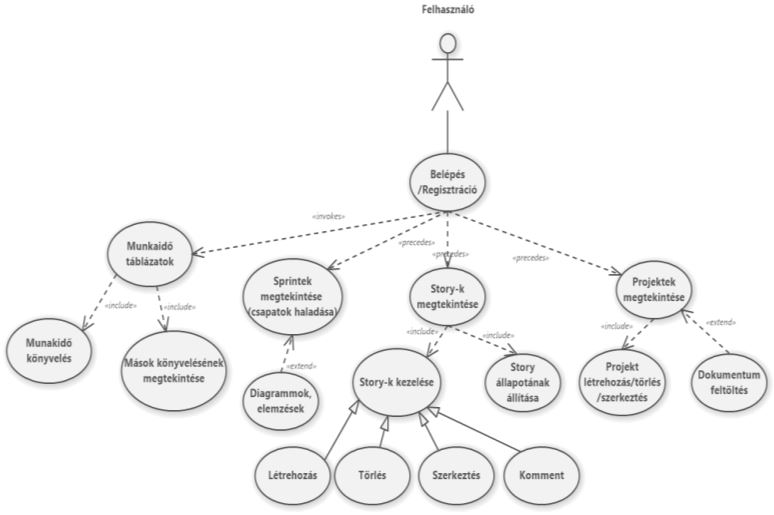
\includegraphics[width=1\textwidth,height=300px]{usecase}
	\caption{Felhasználói eset diagram}
	\label{fig:usecase}
\end{figure}

\section{Struktúrális felépítés}

A ScrumHelper egy MVC (Model-View-Controller) alkalmazás, bár a hivatalos Django dokumentációban az MTV (Model-Template-View) kifejezést használják, mivel ezt gondolják pontosabb leírásának. Tekintve, hogy Djangoban írodott az alkalamzás, ezért ebben a dokumentációban is utóbbi analógia a mérvadó. Ez azt jelenti, hogy három rétegből tevődik össze: egy Model rétegből, amely az adatbázist hivatott reprezentálni, egy View rétegből, amely az adatot reprezentálja (ez alatt azt értjük, amit az adatbázisből kigyűjtött, nem feltétlenül a felhasználó számára megjelnített adatot), valamint a különböző template-ek renderelését is végzi, továbbá egy Template rétegből, mely leírja, hogyan legyen az adat megjelenítve a felhasználó számára.

\begin{figure}[H]
	\centering
	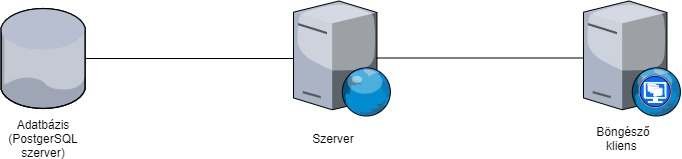
\includegraphics[width=1\textwidth,height=125px]{architecture}
	\caption{Az alkalamzás rétegei: egy adatbázis, egy szerver, ami kinyeri belőle az adatot és továbbítja a nézetnek, valamint a nézet amit a böngészőben láthatunk.}
	\label{fig:architecture}
\end{figure}

A django alkalmazások úgynevezett applikációkból állnak, amelyek a moduláris felépítést segítik elő. Ezek gyakorlatilag a python nyelvből ismert csomagokkal -package-ekkel- egyeznek meg. A \ref{fig:packages}. ábra szemléletesebben bemutatja ezen applikációkat (modulokat) és azok kapcsolatait:

\begin{figure}[H]
	\centering
	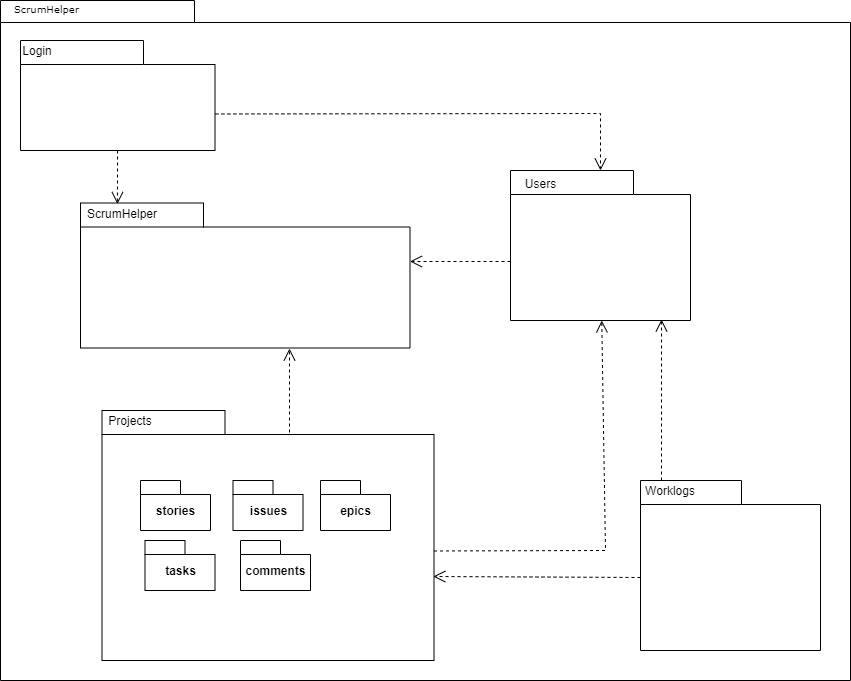
\includegraphics[width=1\textwidth,height=300px]{scrumhelperPackage}
	\caption{Csomagdiagramm}
	\label{fig:packages}
\end{figure}

\pagebreak

\begin{itemize}
 	\item Ahogy az ábrán is látható, a fő csomag a ScrumHelper. Ez fogja össze működésben az alkalamzást.
	\item A legnagyobb applikáció a "Projects", ugyanis ez tartalmazza egyben a "Stories", "Tasks", "Issues", "Comments", "Epics" applikációkat is.
	\item A felhasználók kezelésével foglalkozó csomag a "Users" és részben a "Login". Utóbbi a ki- és bejelentkeztetésre, valamint a felhasználók regisztrálására és szerkeztésére szolgál.
	\item Egy kisebb alkalmazás, a "Worklogs" adja a modell szintű reprezentációját a munkaidő naplónak.
\end{itemize}

Ezek implementáció, részletei a későbbi alfejezetekben olvashatóak. 

\section{Adatbázis réteg}
\label{dbmodels}

A django keretrendszernek köszönhetően az alapkonfigurációt leszámítva nem számít, hogy milyen adatbázissal dolgozunk. A ScrumHelper fejelsztése során a nyílt-forráskódú PostgreSQL-re esett a választás, de a python modellek és az adatbázis lekérdezések függetlenek attól, hogy milyen adatbázist használunk. Ha csak egy kis, egyszerű alkalmazás megvalósítása a cél akkor érdemesebb például SQLite adatbázist használni, tekintve, hogy az csak egy lokális fájlban tárolja az adatokat, könnyebb menedzselni. A PostgreSQL (a MySQL, Oracle, MariaDB mellett) jobb döntésnek bizonyul nagyobb méretű alkalmazások esetén. 

Az egyes adatbázis táblákat (entitásokat) egy-egy modell reprezentál a forráskódban. Ezek a django.db.models.Model osztályból vannak származtatva. Az egyes modellek attribútumai egy-egy oszlopot reprezentálnak a táblában. A django dokumentációban\footnote{django model típusosztályok: \url{https://docs.djangoproject.com/en/3.0/ref/models/fields/}} részletes leírás található arról, mely mezőtípusokhoz milyen paramétereket lehet megadni ahhoz, hogy minél jobban testreszabhassuk a mező tulajdonságait. Van lehetőség modell szintű metódusokat is definiálni ugyanúgy, mint a python osztályoknál (hiszen ezek is python osztályok), de ezek nem lesznek jelen az adatbázisban. A model szinten jellemzően csak egyszerűbb metódusokat szokás definiálni, mint például az \textit{\_\_str\_\_()} felüldefiniálása a felsőbb rétegek segítségéül, vagy az \textit{\_\_init\_\_} inicializációs függényt. Érdemes azonban kerülni az ilyen megoldásokat, hogy minél jobban elszeparálhatóak legyenek az egyes rétegek.  A következő alfejezetekben részletes információk találhatóak az egyes modellekről.

\subsection{Felhasználó kezelés: Users, Login modellek}

\begin{figure}[H]
	\centering
	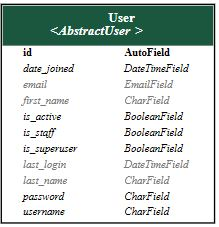
\includegraphics[scale=1.5]{userModel}
	\caption{User modell diagrammja}
	\label{fig:usermodel}
\end{figure}

A \textbf{django.contrib.auth.models.User} model reprezentál egy-egy felhasználót. Ez magában a keretrendszerben megtalálható. Elég sokoldalú, de van lehetőség kiegészíteni, esetlegesen helyettesíteni saját megvalósítással is. Kiegészítésre példa a \textbf{Profile} model osztály a users applikációban. Egy \textbf{OneToOneField} segítségével és szignálokkal (\textit{create\_user\_profile} és \textit{save\_user\_profile}) tudjuk az eredeti \textbf{Users} osztályhoz kötni. A szignálok azért szükségesek, mert így tud a modell reagálni az eredeti modell esetleges változásaira (létrehozás, módosítás, törlés). A mezők:

\begin{itemize}
	\item \textit{id}: mezőazonosító (alapvetően generált)
	\item \textit{date\_joined}: beregisztrálás dátuma
	\item \textit{email}: email cím
	\item \textit{first\_name}: keresztnév
	\item \textit{is\_active}: nem zárolt-e a felhasználó (azaz inaktív)
	\item \textit{is\_staff}: adminisztrátor-e
	\item \textit{is\_superuser}: Minden jogosultsággal rendelkező felhasználó-e
	\item \textit{last\_login}: utolsó bejelentkezés dátuma
	\item \textit{last\_name}: vezeték név
	\item \textit{password}: jelszó (hashelve, azaz kódolva)
	\item \textit{username}: felhasználónév
\end{itemize}

A \textbf{Login} modul nem rendelkezik külön adatbázis reprezentációval, mivel a \textbf{User} modelljét használja föl.

\subsection{Projekt modell}

\begin{figure}[H]
	\centering
	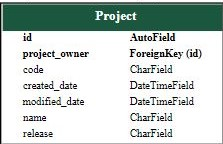
\includegraphics[scale=1.5]{projectModel}
	\caption{Project modell diagrammja}
	\label{fig:projectmodel}
\end{figure}

A \textbf{Projects} applikáció saját adatbázis modellje a \textbf{Project}:

\begin{itemize}
	\item \textit{id}: mezőazonosító (alapvetően generált)
	\item \textit{project\_owner}: a projektet létrehozó felhasználó (idegen kulcs a \textbf{Users} táblára)
	\item \textit{code}: a projekt 6 karakter hosszú kódja (egyedi kell legyen)
	\item \textit{created\_date}: a létrehozás dátuma
	\item \textit{modified\_date}: az utolsó módosítás dátuma
	\item \textit{name}: a projekt neve (maximum 50 karakter hosszú)
	\item \textit{release}: a Release neve (maximum 10 karakter hosszú)
\end{itemize}

Rendelekezik egy \textit{documents} attribútummal is, mely egy \textbf{ManyToManyField} típusú mező, azaz több idegen kulcs kapcsolatot fog egybe (erre a célra a django automatikusan létrehoz egy táblát, amelyben benne lesznek ezek az összekapcsolások) a \textbf{Documents} model táblájának \textit{id} mezőjével. Ennek seígtségével kapcsolódik egy adott projekthez több dokumentum is.

\begin{figure}[H]
	\centering
	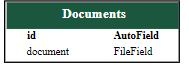
\includegraphics[scale=1.5]{documentModel}
	\caption{Documents modell diagrammja}
	\label{fig:docmodel}
\end{figure}

A \textbf{Documents} model rendelkezik egy \textit{document} attribútummal, mely \textbf{FileField} típusú. Ez a típusosztály reprezentálja Djangoban a fájl mezőket az adatbázisban. A fájl relatív elérési útját menti le az adatbázisba. Jelen alkalmazásban a \textit{documents/} mappát használja, de ez is konfigurálható a \textit{projects.models.project\_directory\_path(instance, filename)} függvény segítségével. A visszatérési értékben (amely egy string) lehet megadni az elérési utat.

\subsection{Epic modell}

\begin{figure}[H]
	\centering
	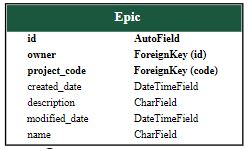
\includegraphics[scale=1.5]{epicModel}
	\caption{Epic modell diagrammja}
	\label{fig:epicmodel}
\end{figure}

Az \textbf{Epic} a \textit{project\_code} mezővel kapcsolódik a \textbf{Project} tábla \textit{code} mezőjéhez. Egy projekthez több több epic is tartozhat, de egy epic csak egy projekthez kapcsolódhat. Ha a projekt törlődik, vagy a létrehozó felhasználó, akkor az összes epic is amelyek hozzá tartoznak. A modell mezői:

\begin{itemize}
	\item \textit{id}: mezőazonosító (alapvetően generált)
	\item \textit{owner}: az epic-et létrehozó felhasználó (idegen kulcs a \textbf{Profile} táblára)
	\item \textit{project\_code}: a projekt 6 karakter hosszú kódja (idegen kulcs, a \textbf{Project} tábla \textit{code} mezőjére mutat)
	\item \textit{created\_date}: a létrehozás dátuma
	\item \textit{modified\_date}: az utolsó módosítás dátuma
	\item \textit{name}: az epic neve (maximum 50 karakter hosszú)
	\item \textit{description}: egy leírás az epic-ről (maximum 250 karakter hosszú)
\end{itemize}

\subsection{Story modellje}

\begin{figure}[H]
	\centering
	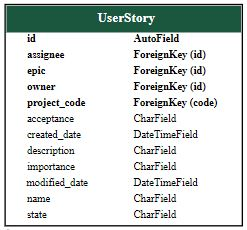
\includegraphics[scale=1.5]{storyModel}
	\caption{Story modell diagrammja}
	\label{fig:storymodel}
\end{figure}

A \textbf{UserStory} több táblához is rendelkezik idegen kulccsal: kapcsolódik egyrészt a projekthez, amely alatt létrehozták, kapcsolódik továbbá a felhasználóhoz, aki létrehozta, illetve akihez rednelve van (utóbbi opcionális), valamint kapcsolódik egy epic-hez (ez is opcionális). Egy story csak addig létezik, amíg a projekt is, amely alatt létehozták, avagy ki nem törlik. Ha epic-hez van rendelve és töröljük, akkor csak kinullázódik azon mezője. Abban az esetben, ha a felhasználót töröljük, aki létrehozta a story-t, akkor is törlődik. A modell mezői:

\begin{itemize}
	\item \textit{id}: mezőazonosító (alapvetően generált)
	\item \textit{assignee}: idegen kulcs a hozzárendelt felhasználóra (lehet üres, \textbf{User} tábla)
	\item \textit{epic}: idegen kulcs az \textbf{Epic} táblára (lehet üres)
	\item \textit{owner}: az story-t létrehozó felhasználó (idegen kulcs a \textbf{Profile} táblára)
	\item \textit{project\_code}: a projekt 6 karakter hosszú kódja (idegen kulcs, a \textbf{Project} tábla \textit{code} mezőjére mutat)
	\item \textit{acceptance}: feltételek leírása, amelyeknek teljesülnie kell (például teszt során, maximum 50 karakter)
	\item \textit{created\_date}: a létrehozás dátuma
	\item \textit{modified\_date}: az utolsó módosítás dátuma
	\item \textit{name}: az epic neve (maximum 50 karakter hosszú)
	\item \textit{description}: egy leírás a story-ról (maximum 250 karakter hosszú)
	\item \textit{importance}: fontosság (Low, Medium, High)
	\item \textit{state}: aktuális állapot (OPEN, IN PROGRESS, TESTING, DONE, CLOSED)
\end{itemize}

\subsection{Task modellje}

\begin{figure}[H]
	\centering
	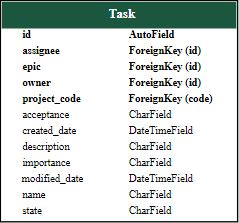
\includegraphics[scale=1.5]{taskModel}
	\caption{Task modell diagrammja}
	\label{fig:taskmodel}
\end{figure}

